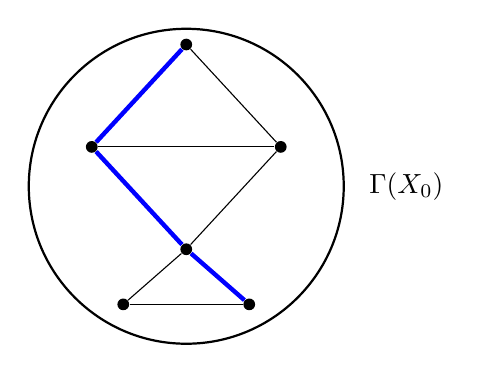
\begin{tikzpicture}
    % Sphere (represented as a circle)
    \draw[thick] (0,0) circle (2cm);
    
    % Triangulation points
    \node (p1) at (0, 1.8) [circle, fill, inner sep=1.5pt] {};
    \node (p2) at (-1.2, 0.5) [circle, fill, inner sep=1.5pt] {};
    \node (p3) at (1.2, 0.5) [circle, fill, inner sep=1.5pt] {};
    \node (p4) at (0, -0.8) [circle, fill, inner sep=1.5pt] {};
    \node (p5) at (-0.8, -1.5) [circle, fill, inner sep=1.5pt] {};
    \node (p6) at (0.8, -1.5) [circle, fill, inner sep=1.5pt] {};
    
    % Triangulation edges
    \draw (p1) -- (p2);
    \draw (p1) -- (p3);
    \draw (p2) -- (p3);
    \draw (p2) -- (p4);
    \draw (p3) -- (p4);
    \draw (p4) -- (p5);
    \draw (p4) -- (p6);
    \draw (p5) -- (p6);
    
    % Heavy blue edges for gluing
    \draw[blue, ultra thick] (p1) -- (p2);
    \draw[blue, ultra thick] (p2) -- (p4);
    \draw[blue, ultra thick] (p4) -- (p6);
    
    \node[anchor=west] at (2.2, 0) {$\Gamma(X_0)$};
\end{tikzpicture}
